%%%%%%%%%%%%%%%%%%%%%%%%%%%%%%%%%%%%%%%%%%%%%%%%%%%%%%%%%%%%%%%%%%%%%%
% Relatório técnico para disciplina de Teoria da Computação
%%%%%%%%%%%%%%%%%%%%%%%%%%%%%%%%%%%%%%%%%%%%%%%%%%%%%%%%%%%%%%%%%%%%%%

\documentclass[12pt]{article}

\usepackage{float}
\usepackage{sbc-template}
\usepackage{graphicx,url,algorithm,listings}
\usepackage[brazil]{babel}  
\usepackage[utf8]{inputenc}



\usepackage{listings}
\usepackage{xcolor}
\renewcommand{\lstlistingname}{Código}
\lstset{
  basicstyle=\ttfamily,
  breaklines=true,
  frame=single,
  captionpos=b,
  showstringspaces=false,
  keywordstyle=\bfseries,
  numbers=left,
  numberstyle=\tiny
}

\title{Implementação de Autômatos e Transdutores Finitos Determinísticos para Linguagens Regulares e Aplicações}

\author{Christian Amarildo Amorim Morais\inst{1} \\ 
        Daniel Naiff da Costa\inst{2} \\
        Gabriel Lemos da Silva Mastub\inst{3} \\
        Raiane Gabriele Brito de Oliveira \inst{4} \\
        Rogério dos Anjos Barbosa \inst{5} \\}

\address{Universidade Federal do Pará\\
Instituto de Ciências Exatas e Naturais\\
Bacharelado em Ciência da Computação\\
Belém -- PA -- Brasil
\email{christian.morais@icen.ufpa.br}
\email{raiane.oliveira@icen.ufpa.br}
\email{rogerio.barbosa@icen.ufpa.br}
\email{colocar outros emails aqui}
}

\renewcommand{\lstlistingname}{Código}

\begin{document}

\maketitle

\begin{abstract}
    This article addresses the resolution of a list of questions and the implementation of deterministic finite automata (DFAs) for regular languages and finite transducers (Mealy Machines). The work focuses on pattern recognition, input data processing, and the simulation of interactions, such as the dispensing of sodas based on coin insertion. The article is structured into an introduction, materials and methods, experimental tests, and final remarks.
\end{abstract}

\begin{resumo}
  Este artigo aborda a resolução de uma lista de questão e a implementação de autômatos finitos determinísticos (AFDs) para linguagens regulares e transdutores finitos (Máquinas de Mealy). O trabalho foca no reconhecimento de padrões, processamento de entrada de dados e simulação de interações, como a entrega de refrigerantes com base na inserção de moedas. O artigo está estruturado em introdução, materiais e métodos, testes experimentais e comentários finais.
\end{resumo}

\section{\textbf{Introdução}}

A Teoria da Computação tem como foco o estudo das linguagens formais e os mecanismos capazes de reconhecê-las, sendo uma área fundamental da ciência da computação. Autômatos finitos determinísticos (AFDs) são modelos matemáticos que reconhecem linguagens regulares e são amplamente utilizados em tarefas como validação de entrada de dados, análise lexical e controle de sistemas. Além disso, transdutores finitos, como as Máquinas de Mealy e Moore, são usados para modelar sistemas interativos, processando entradas e gerando saídas.

Este trabalho apresenta a implementação de autômatos que reconhecem linguagens regulares, definidas por expressões regulares, e um transdutor finito que simula a entrega de refrigerantes a partir da inserção de moedas.

\section{\textbf{Materiais e Métodos}}

Neste artigo, utilizamos a linguagem de programação Python devido a sua simplicidade e recursos que facilitam na manipulação de expressões regulares e autômatos. As bibliotecas padrão de Python, tais como a "re" "regex" "AutomataLib" "pyformlang" "networkx" "FiniteStateMachine" "FSM", também, foram levadas em consideração na escolha da linguagem e na produção das implementações . 

Cada autômato, Regex e transdutor foi desenvolvido seguindo as instruções e delimitações do comando de cada questão, fazendo isso da melhor forma possível, utilizando o Jflap para a melhoria da imagem do automato final.

\subsection{Questão 1.a) Linguagem \((ab^*c^*)^*\)}

A linguagem da expressão regular da "questão 1.a" esta representando cadeias que começam com o símbolo `a` seguido de zero ou mais `b`s e zero ou mais `c`s, repetidas múltiplas vezes. Abaixo está a implementação do autômato final no "Jflap":

\begin{figure}[H]
\centering
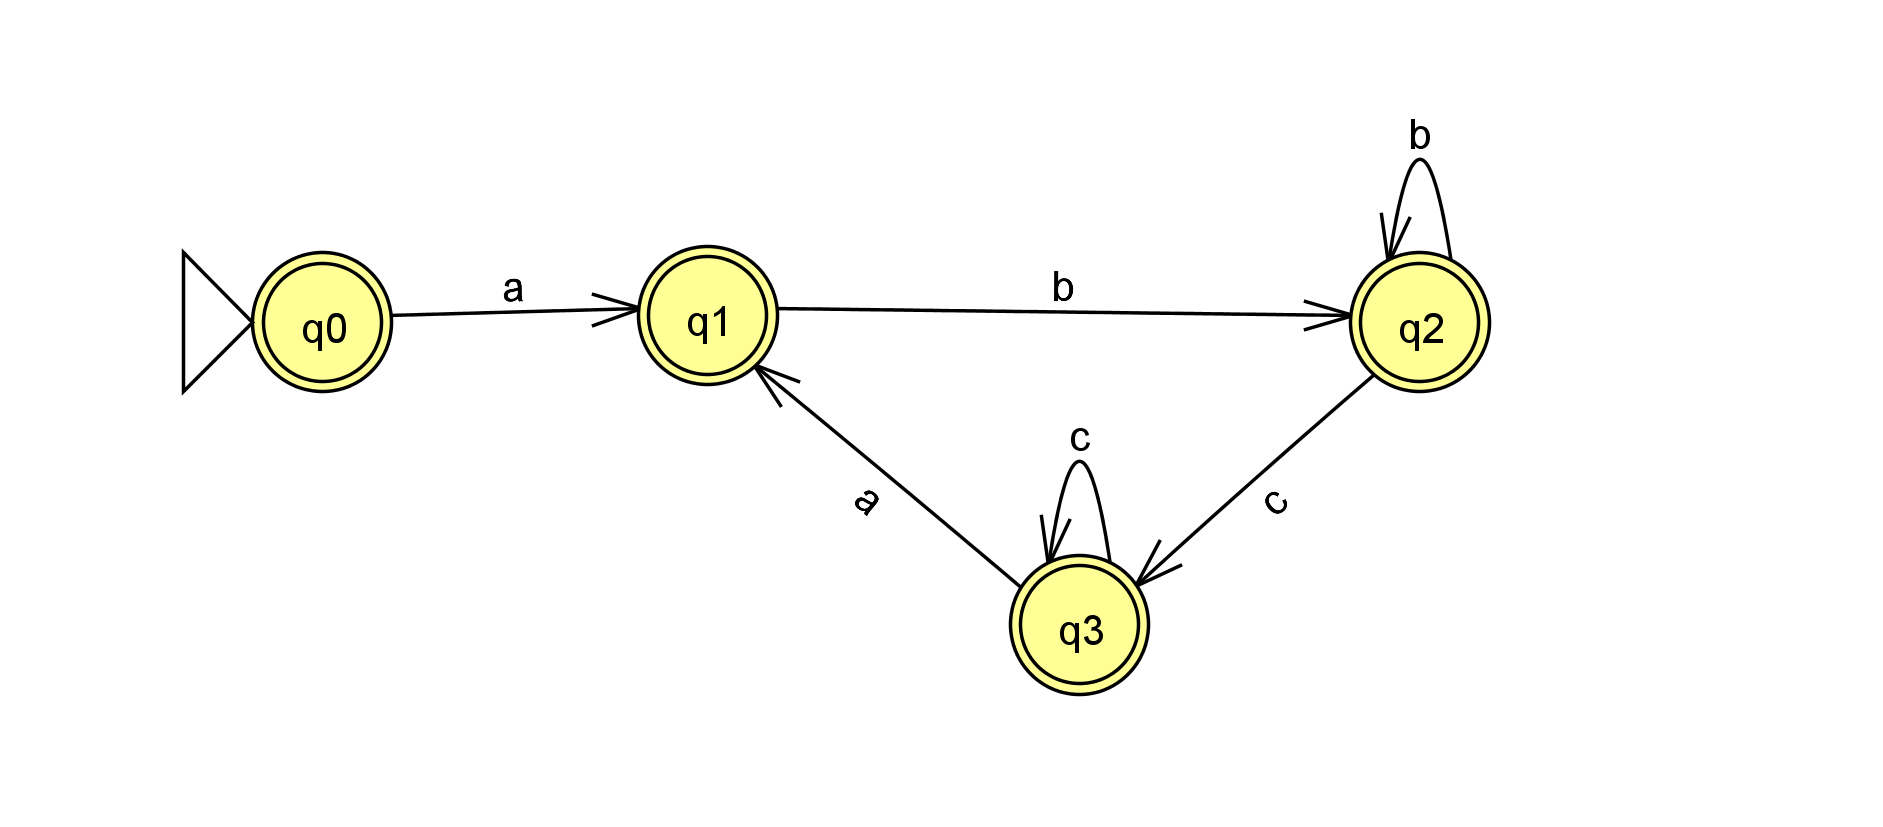
\includegraphics[width=1\textwidth]{questao1/output/questao 1 automatos.png} 
\caption{ Autômato para a linguagem da questão 1.a gerado no JFLAP}
\label{fig:regexExplanation}
\end{figure}


\subsection{Questão 1.b) Linguagem \(aaa(b | c)^* | (b | c)^* aaa\)}

A linguagem da expressão regular da "questão 1.b" esta representando cadeias que começam ou terminam com a sequência `aaa`, seguidas ou precedidas de uma sequência arbitrária de `b`s ou `c`s.

\begin{figure}[H]
\centering
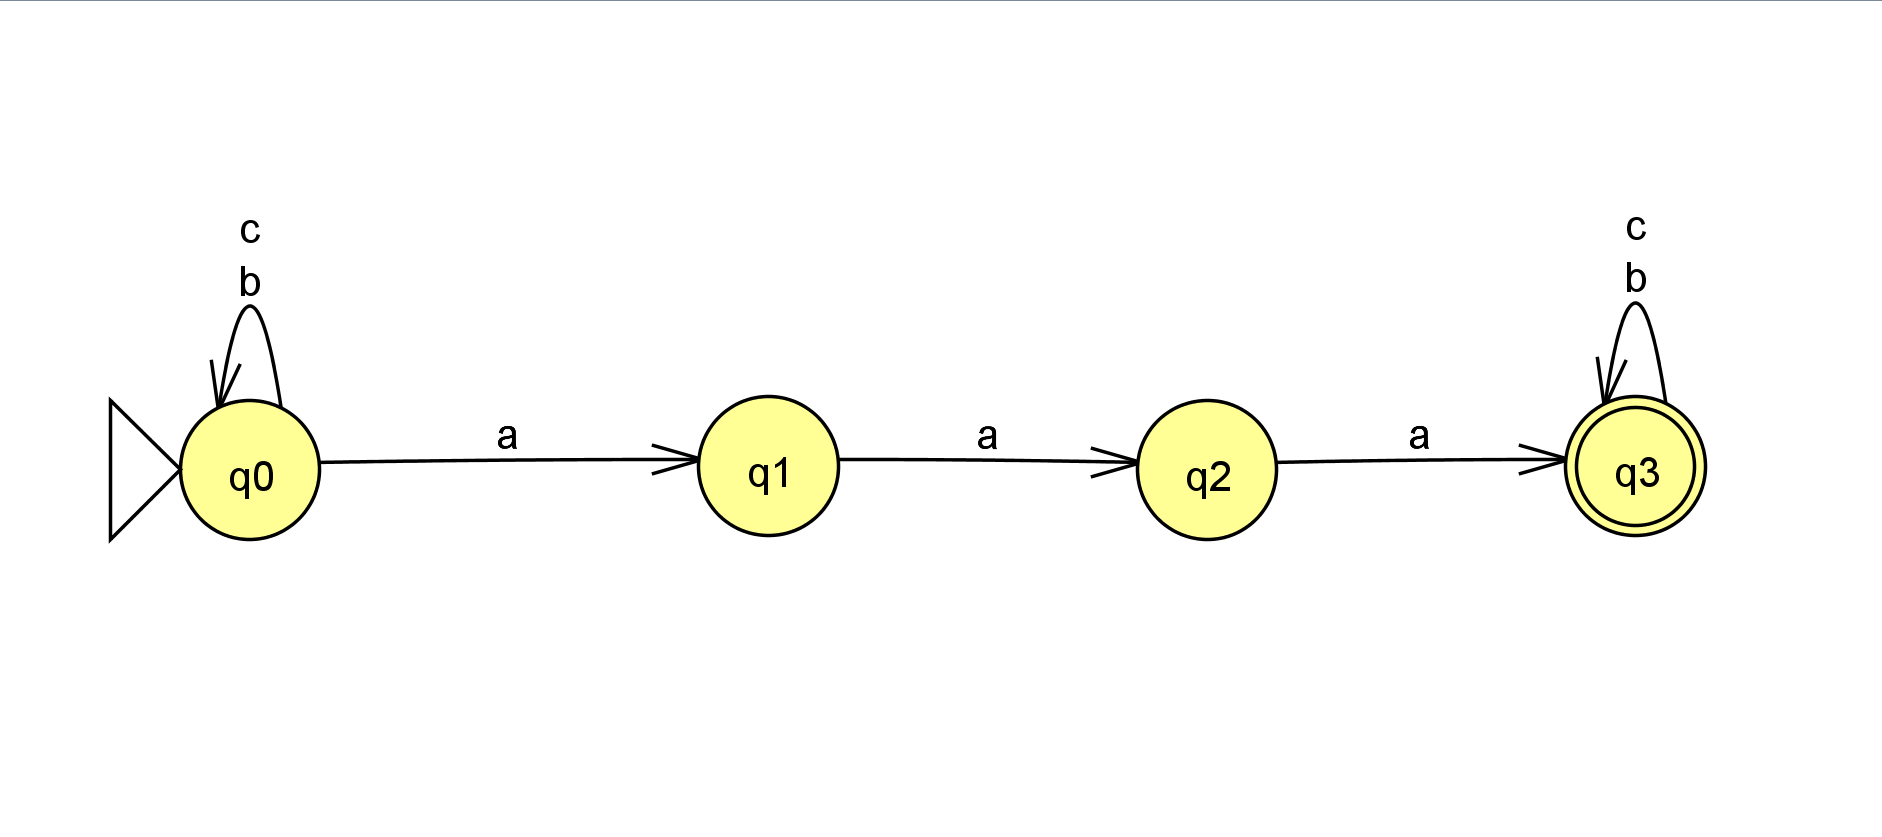
\includegraphics[width=1\textwidth]{questao1/output/questao 2 automatos.png} 
\caption{Autômato para a linguagem da questão 1.b gerado no JFLAP}
\label{fig:regexExplanation}
\end{figure}

\subsection{Questão 1.c) Linguagem \(a^*b | ab^*
\)}

A linguagem da expressão regular da "questão 1.c" esta representando cadeias que começam com zero ou mais `a`s, seguidas de um `b`, ou começa com um "a" e terminam com zero ou mais `b`s.

\begin{figure}[H]
\centering
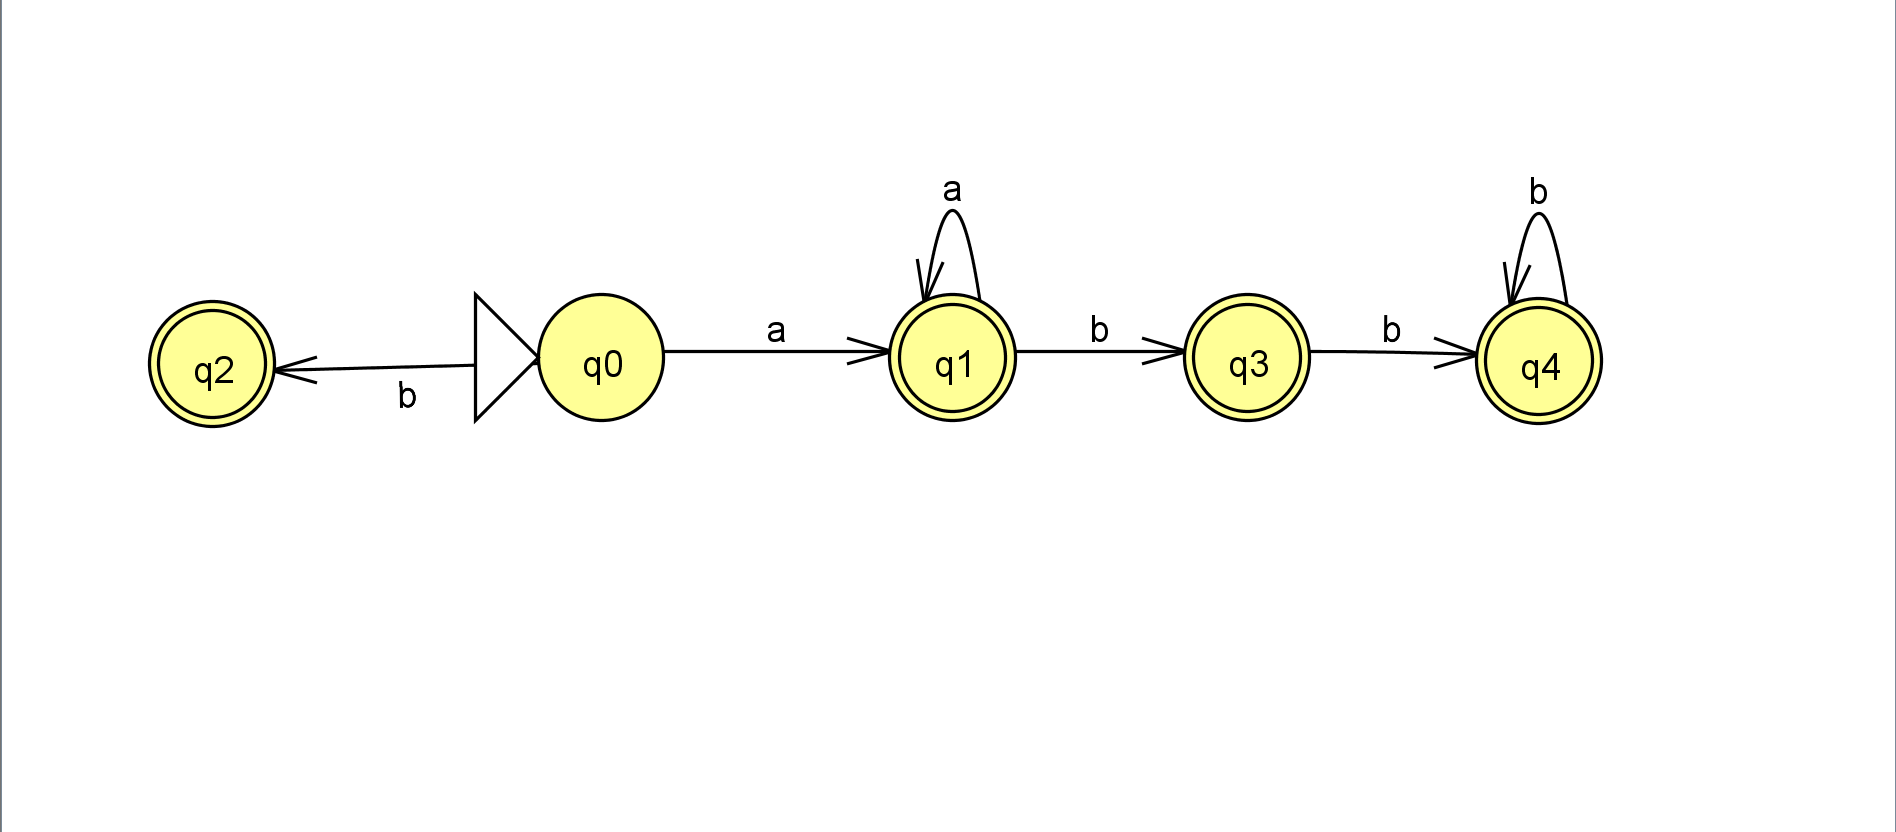
\includegraphics[width=1\textwidth]{questao1/output/questao 3 automatos.png} 
\caption{Autômato para a linguagem da questão 1.c gerado no JFLAP}
\label{fig:regexExplanation}
\end{figure}

\subsection{Questão 1.d) Linguagem \(a^*b^*(a | ac^*)\)}

A linguagem da expressão regular da "questão 1.d" esta representando cadeias que começam com zero ou mais `a`s, seguidas de zero ou mais `b`s, e terminam com um `a` ou `ac*`.

\begin{figure}[H]
\centering
\includegraphics[width=1\textwidth]{questao1/output/questao 4 automatos.png} 
\caption{Autômato para a linguagem da questão 1.d gerado no JFLAP}
\label{fig:regexExplanation}
\end{figure}

\subsection{Questão 2: Autômato finito que reconhece as ocorrências da cadeia "computador" no texto da questão.}

\begin{figure}[H]
\centering
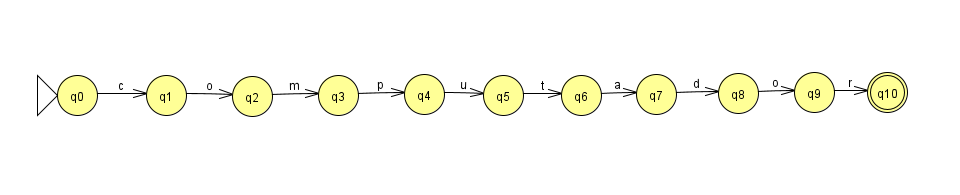
\includegraphics[width=1.1\textwidth]{questao2/output/Questão 2 autômato.png} 
\caption{Autômato para a questão 2}
\label{fig:regexExplanation}
\end{figure}

De acordo com as especificações da questão 2, foi criado o autômato finito, que reconhece a cadeia "computador", representado pela Figura 5. O autômato é composto por 11 estados que fazem parte do conjunto $Q$ = \{'q0', 'q1', 'q2', 'q3', 'q4', 'q5', 'q6', 'q7', 'q8', 'q9', 'q10'\}, o seu estado inicial é o estado '$q_0$', o conjunto dos estados finais é composto apenas pelo estado denominado de 'q10', $F$ = \{'q10'\}, o seu alfabeto é composto pelos caracteres que formam a palavra "computador", ou seja, fazem parte do conjunto $\Sigma$ = \{'c', 'o', 'm', 'p', 'u', 't', 'a', 'd', 'o', 'r'\} e as funções de transições são representadas pelo conjunto $\delta$ = \{(q0,'c') → q1, (q1,'o') → q2, (q2,'m') → q3, (q3,'p') → q4, (q4,'u') → q5, (q5,'t') → q6, (q6,'a') → q7, (q7,'d') → q8, (q8,'o') → q9, (q9,'r') → q10 \}.


\begin{lstlisting}[style=Python, caption={Código da classe 'AutomatoFinito' da questão 2}]

\end{lstlisting}

Para implementar o autômato da figura 5 foi usado uma classe chamada 'AutomatoFinito', como é possível ver no código 1. Essa classe possui atributos chamados 'estados', 'alfabeto', 'transições', 'estado\_inicial' e 'estados\_finais' que armazenam respectivamente os conjuntos  $Q$, $\Sigma$, $\delta$, $q_0$ e $F$.

Ainda, no código 1, classe possui o método chamado 'separarPalavras' que processa o texto dado da questão e separa cada palavra e armazena em uma lista retirando os espaços e pontos e o método 'processar' que é responsável por aplicar as especificações do autômato no texto. Na linha 15 a captura a lista de palavras, na linha 17 é criada uma lista para armazenar as cadeias reconhecidas, em seguida dentro do loop, na linha 23, inicia-se o estado inicial e a partir da linha 24 é criado outro loop que verifica letra por letra, da lista de palavras separadas, se está contido na função de transição. Após a verificação de todas as letras da palavra, na linha 32, é verificado se o estado em questão é o final, caso positivo é adicionado a cadeia na lista 'palavras\_reconhecidas' e também é adicionado a sua posição na lista 'posições'.

\begin{lstlisting}[style=Python, caption={Código da implementação de teste da questão 2}]

\end{lstlisting}

No código 2, foi implementado a parte do código que realiza a execução dos métodos da classe do código 1. Primeiramente foi implementada uma função chamada 'destacar\_palavras' que tem a finalidade de destacar as cadeias aceitas em verde no texto, isso foi adicionado para facilitar a visualização do professor. A função tem como parâmetros o 'texto', 'posições' e 'palavras', que representam respectivamente o texto que a questão pede para processar, as posições que foram encontradas pelo método da classe, do código 1, e as palavras reconhecidas pelo autômato. Essa função iterar sobre as posições das palavras reconhecidas e muda de cor caso essa condição da linha 52 'texto[pos:pos + len(palavra)] == palavra' seja atendida.

Na linha 63 até a linha 78 é dado os conjuntos do autômato. Na linha 80 é criado o objeto 'autômato' e incializado os seu atributos através do construtor. Na linha 82 é dado o texto da questão e da linha 90 até a linha 97 é usado os métodos do objeto e finalmente é apresentado os resultados para o usuário.

\subsection{Questão 3: Transdutor Finito para Entrega de Refrigerantes}

Na questão 3, o transdutor foi implementado como uma Máquina de Mealy que processa a inserção de moedas (25, 50 centavos e 1 real) e libera uma lata de refrigerante quando o valor totaliza 1 real ou mais. A saída será `0` enquanto o valor não for suficiente e `1` quando a lata for liberada.

\begin{figure}[H]
\centering
\includegraphics[width=1.1\textwidth]{images/questao 3 mealy.pdf} 
\caption{Autômato para a questão 3}
\label{fig:regexExplanation}
\end{figure}

Na figura 6, há um autômato com 4 estados que fazem parte do conjunto $Q$ = \{'q0', 'q1', 'q2', 'q3'\}, com o estado inicial sendo "q0", onde cada um deles está representando a acumulação do dinheiro na máquina. O alfabeto de entrada deste autômato é composto pelo conjunto $\Sigma$ = \{'25', '50', '100'\} (representam as moedas que a máquina irá receber de entrada) e o alfabeto de saída é composto pelo conjunto $\Delta$ = \{'1'\} (representa a saída de um refrigerante da máquina). A função de transição do autômato é $\delta$ = \{(q0, '25') → q1, (q0, '50') → q2, (q0, '100') → q0, (q1, '25') → q2, (q1, '50') → q3, (q1, '100') → q1, (q2, '25') → q3, (q2, '50') → q0, (q2, '100') → q2, (q3, '25') → q0, (q3, '50') → q1, (q3, '100') → q3\} e a função de transdução é $\lambda$ = \{(q0, '25') → $\epsilon$, (q0, '50') → $\epsilon$, (q0, '100') → '1', (q1, '25') → $\epsilon$, (q1, '50') → $\epsilon$, (q1, '100') → '1', (q2, '25') → $\epsilon$, (q2, '50') → '1', (q2, '100') → '1', (q3, '25') → '1', (q3, '50') → '1', (q3, '100') → '1'\}. 

Ainda na figura 6, o estado "q0" acumula 0 centavos, "q1" acumula 25 centavos, "q2" acumula 50 centavos e "q3" acumula 75 centavos, não ultrapassando 1 real (ou 100 centavos), pois ao chegar nesse valor, a máquina libera um refrigerante e a acumulação reinicia (ou seja, a acumulação significa o quanto ultrapassou de dinheiro na máquina desde a última liberação de um refrigerante), e dependendo do valor inserido, a acumulação pode mudar para um estado (ou seja, mudar de valor acumulado) ou permanecer em seu estado atual.

\begin{lstlisting}[style=Python, caption={Código do autômato da questão 3}]
def Mealy(estados, alfabeto_entrada, alfabeto_saida, transicao, transducao, estado_inicial, cadeia):
     qTs = estado_inicial
     sTd = ''
     ss = ''
     for s in cadeia:
          ss = ss + s
          if ss == '25' or ss == '50' or ss == '100':
               sTd = sTd + transducao[(qTs, ss)]
               qTs = transicao[(qTs, ss)]
               ss = ''
     return sTd
\end{lstlisting}

De acordo com as especificações da questão, no código 3 foi necessário implementar uma função chamada "Mealy()", que recebe os argumentos "estados", "alfabeto\_entrada", "alfabeto\_saída", "transicao", "transducao", "estado\_inicial", que representam respectivamente os conjuntos $Q$, $\Sigma$, $\Delta$, $\delta$, $\lambda$ e $q0$. Além disso, a função receberá um argumento que será a cadeia de entrada para a leitura do autômato.

Continuando no código 3, a função "Mealy()" três variáveis iniciais, uma para a transição de estados (essa variável indicará em qual estado o autômato se encontra), outra variável que irá receber as saídas do autômato, e outra que vai servir para a leitura da cadeia adicionada nos argumentos da função. A variável de leitura percorrerá a cadeia de entrada, e quando ler um valor do conjunto Q = \{'25', '50', '100'\}, a variável de estado será mudada pela função de transição $\delta$, onde também a variável de transição poderá ser mudada a depender da transição e a variável de leitura da cadeia ficará vazia para poder ler outros símbolos e executar novas transições a partir deles. No final, a função vai retornar o valor daquela variável que possuía essa cadeia de saída.

\begin{lstlisting}[style=Python, caption={Função para testar cadeias no autômato da questão 3}]
def testar_cadeias(estados, alfabeto_entrada, alfabeto_saida, transicao, transducao, estado_inicial, vetor_cadeias):
     for c in vetor_cadeias:
          print(f'{c} = {mealy(estados, alfabeto_entrada, alfabeto_saida, transicao, transducao, estado_inicial, c)}')
\end{lstlisting}

Para testar no autômato um vetor contendo múltiplas cadeias, no código 4 foi necessário criar uma função "testar\_cadeias()", que contém os mesmos argumentos presentes na função do código 3, exceto pelo argumento "cadeia", que na função do código 4 foi substituída pelo argumento "vetor\_cadeias", onde é ele que vai receber o vetor que contém as diversas cadeias que serão avaliadas na função. Dentro da função, há uma estrutura de repetição "for" que contém uma variável que vai percorrer o vetor, e a cada iteração, serão imprimidos os resultados para cada cadeia dentro do vetor, visto que dentro da função "print()", há a mesma função presente no código 3.

Agora, abordando outras explicações, as funções de transição e transdução exigiram a necessidade de serem feitas com dicionários, onde dentro dos parênteses temos a cadeia atual e o símbolo de leitura, e fora dos parênteses temos o estado atual do autômato (para a função de transição) e a impressão da transição (para a função de transdução). Os dicionários eram necessários para fazer esse controle no código 3, pois a partir dos valores de dentro dos parênteses, poderíamos determinar os valores das variáveis que receberão o estado atual do autômato e a impressão feita nas transições.

\section{\textbf{Testes Experimentais}}

A seguir, os testes realizados para validar as implementações dos autômatos e do transdutor.

\subsection{Testes da Questão 1.a)}

Os testes a seguir foram realizados para validar o reconhecimento de cadeias da linguagem \((ab^*c^*)^*\).

%imagem


\subsection{Testes da Questão 1.b)}

Os testes a seguir foram realizados para validar o reconhecimento de cadeias da linguagem \(aaa(b | c)^* | (b | c)^* aaa\).

%imagem


\subsection{Testes da Questão 1.d)}

Os testes a seguir foram realizados para validar o reconhecimento de cadeias da linguagem \(a^*b^*(a | ac^*)\).

%imagem


\subsection{Testes da Questão 2}

\begin{figure}[H]
\centering
\includegraphics[width=1\textwidth]{questao2/teste/teste questão 2.png} 
\caption{saída no terminal da questão 2}
\label{fig:regexExplanation}
\end{figure}

Na figura 6 é possível ver que o algoritmo dos códigos 1 e 2 foram capazes de  apontar nas posições 2, 133, 294, 412 e 440 que ocorreram o casamento exato da palavra 'computador' e também foram bem sucedidos em destacar a cadeia no texto original para uma melhor visualização do professor.

\subsection{Testes da Questão 3}

\begin{figure}[H]
\centering
\includegraphics[width=1\textwidth]{images/testes questao 3.pdf} 
\caption{saída no terminal da questão 3}
\label{fig:regexExplanation}
\end{figure}

Na figura 7, é possível notar as cadeias de entrada à esquerda, e as cadeias de saída à direita. É possível notar nesta figura que há cadeias que não acumulam 100 centavos, como a '25' e a '2550', portanto imprimem vazio na tabela, ou seja, a máquina não liberou nenhum refrigerante. Já outras cadeias imprimem o símbolo '1' uma vez ou repetidas vezes, pois estas acumularam 100 centavos uma ou mais de uma vez, e entre elas é possível notar que há cadeias que, apesar de acumularem algumas vezes os 100 centavos, há uma parte do dinheiro sobrando, como é o caso da '505050' e da '2525252525252525', onde a máquina ainda possui um montante de dinheiro que ainda não acumulou o suficiente para liberar mais um refrigerante.

\section{\textbf{Comentários Finais}}

Os testes experimentais indicaram que as implementações funcionaram conforme o esperado. As cadeias que pertenciam às linguagens foram corretamente aceitas pelos autômatos, enquanto as cadeias que não pertenciam foram rejeitadas. No caso do transdutor, ele liberou corretamente as latas de refrigerante quando o valor total de moedas atingiu ou superou 1 real.

As implementações demonstram a aplicabilidade dos autômatos finitos determinísticos para o reconhecimento de linguagens regulares e de transdutores finitos em sistemas interativos simples. A escolha da linguagem Python facilitou a implementação e a manipulação de expressões regulares, garantindo a clareza e eficiência dos resultados obtidos.

\appendix

\section{Código-Fonte}

O código completo das implementações pode ser acessado no seguinte repositório:

\url{https://github.com/exemplo-repositorio/automatos.git}

\end{document}
